\tikzstyle{startstop} = [rectangle, rounded corners, minimum width=3cm, minimum height=1cm, text centered, draw=black, fill=red!30]
\tikzstyle{io} = [trapezium, trapezium left angle=70, trapezium right angle=110, minimum width=3cm, minimum height=1cm, text centered, draw=black, fill=blue!30]
\tikzstyle{process} = [rectangle, minimum width=2.5cm, minimum height=1cm, text centered, draw=black, fill=orange!30, text width=6cm]
\tikzstyle{decision} = [diamond, minimum width=3cm, minimum height=1cm, text centered, draw=black, fill=green!30]
\tikzstyle{seta}  = [thick,->,>=stealth]

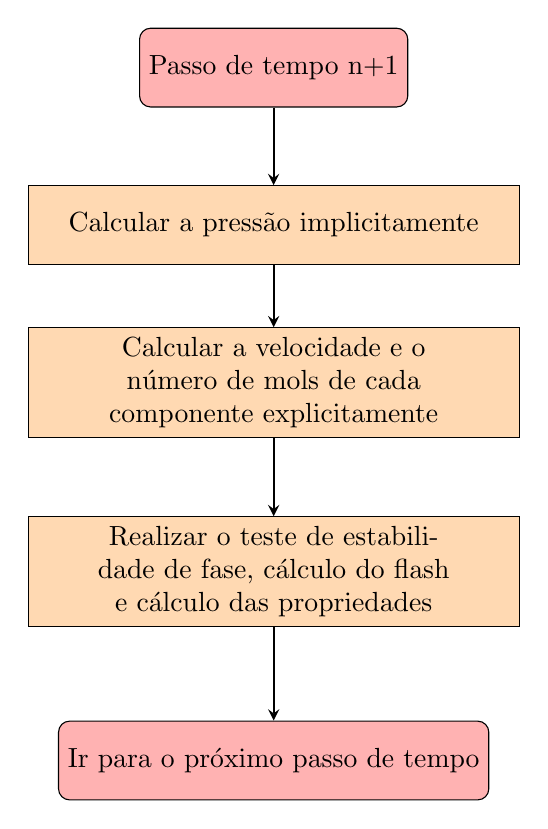
\begin{tikzpicture}[node distance=2cm]

  \node (start) [startstop] {Passo de tempo n+1};
  \node (proc0) [process, below of=start] {Calcular a pressão implicitamente};
  \node (proc1) [process, below of=proc0] {Calcular a velocidade e o número de mols de cada componente explicitamente};
  \node (proc2) [process, below of=proc1, yshift=-0.4cm] {Realizar o teste de estabilidade de fase, cálculo do flash e cálculo das propriedades};
  \node (end) [startstop, below of=proc2,yshift=-0.4cm] {Ir para o próximo passo de tempo};
  
  
  \draw[seta] (start) -- (proc0);
  \draw[seta] (proc0) -- (proc1);
  \draw[seta] (proc1) -- (proc2);
  \draw[seta] (proc2) -- (end);
  % \draw[seta] (proc3) -- (proc4);
  % \draw[seta] (proc4) -- (proc5);
  % \draw[seta] (proc5) -- (dec1);
  % \draw[seta] (dec1) -- node[anchor=east]{Sim} (end);
  % \draw[seta] (dec1) -- node[anchor=south]{Não} (proc6);
  % \draw[seta] (proc6) -- (proc7);
  % \draw[seta] (proc7) -- (proc8);
  % \draw[seta] (proc8) -- (dec2);
  % \draw[seta] (dec2) -- node[anchor=west]{Sim} (proc9);
  % \draw[seta] (dec2) -- coordinate[midway](m1) node[anchor=north]{Não} (proc2);
  % \draw[seta] (proc9) -| (m1);
\end{tikzpicture}
